\section{Introduction}
\label{sec:intro}
\IEEEPARstart{M}{icrophones} are widely embedded in commercial electric device nowadays, which intensifies concerns over voice privacy. As shown in Figure~\ref{fig:introduction_system}, people are surrounded by various microphone-equipped devices in daily life, such as smartphones and smart speakers. Due to their blackbox nature, it is possible for adversaries to exploit, compromise, or even misconfigure these devices for eavesdropping. With the help of automatic speech recognition (ASR) systems, victims' personal data could be extracted thus violating their privacy. Many news reports the risk of being eavesdropped all the time by devices equipped with Siri, Alexa, or Google Assistant~\cite{android_police,alexa_google,siri}. Some reported cases also show severe consequences caused by eavesdropping:
In 2021, a leaked recording says that the Revolutionary Guards Corps overruling many government decisions, which puts the speaker in the recording, the Foreign Minister of Iranian, into a particular point of contention~\cite{iran_foreign_minister}. In 2020, the Ukraine prime minister submitted his resignation because a leaked recording suggesting he had criticized the president~\cite{GuardianUkraine}. In 2018, the defense secretary of the UK was interrupted by voice assistant during Commons statement because Siri listens constantly to seek the wake word~\cite{BBCSiri}, which can be treated as a new form of eavesdropping. 

\begin{figure}[t]
    \centering
    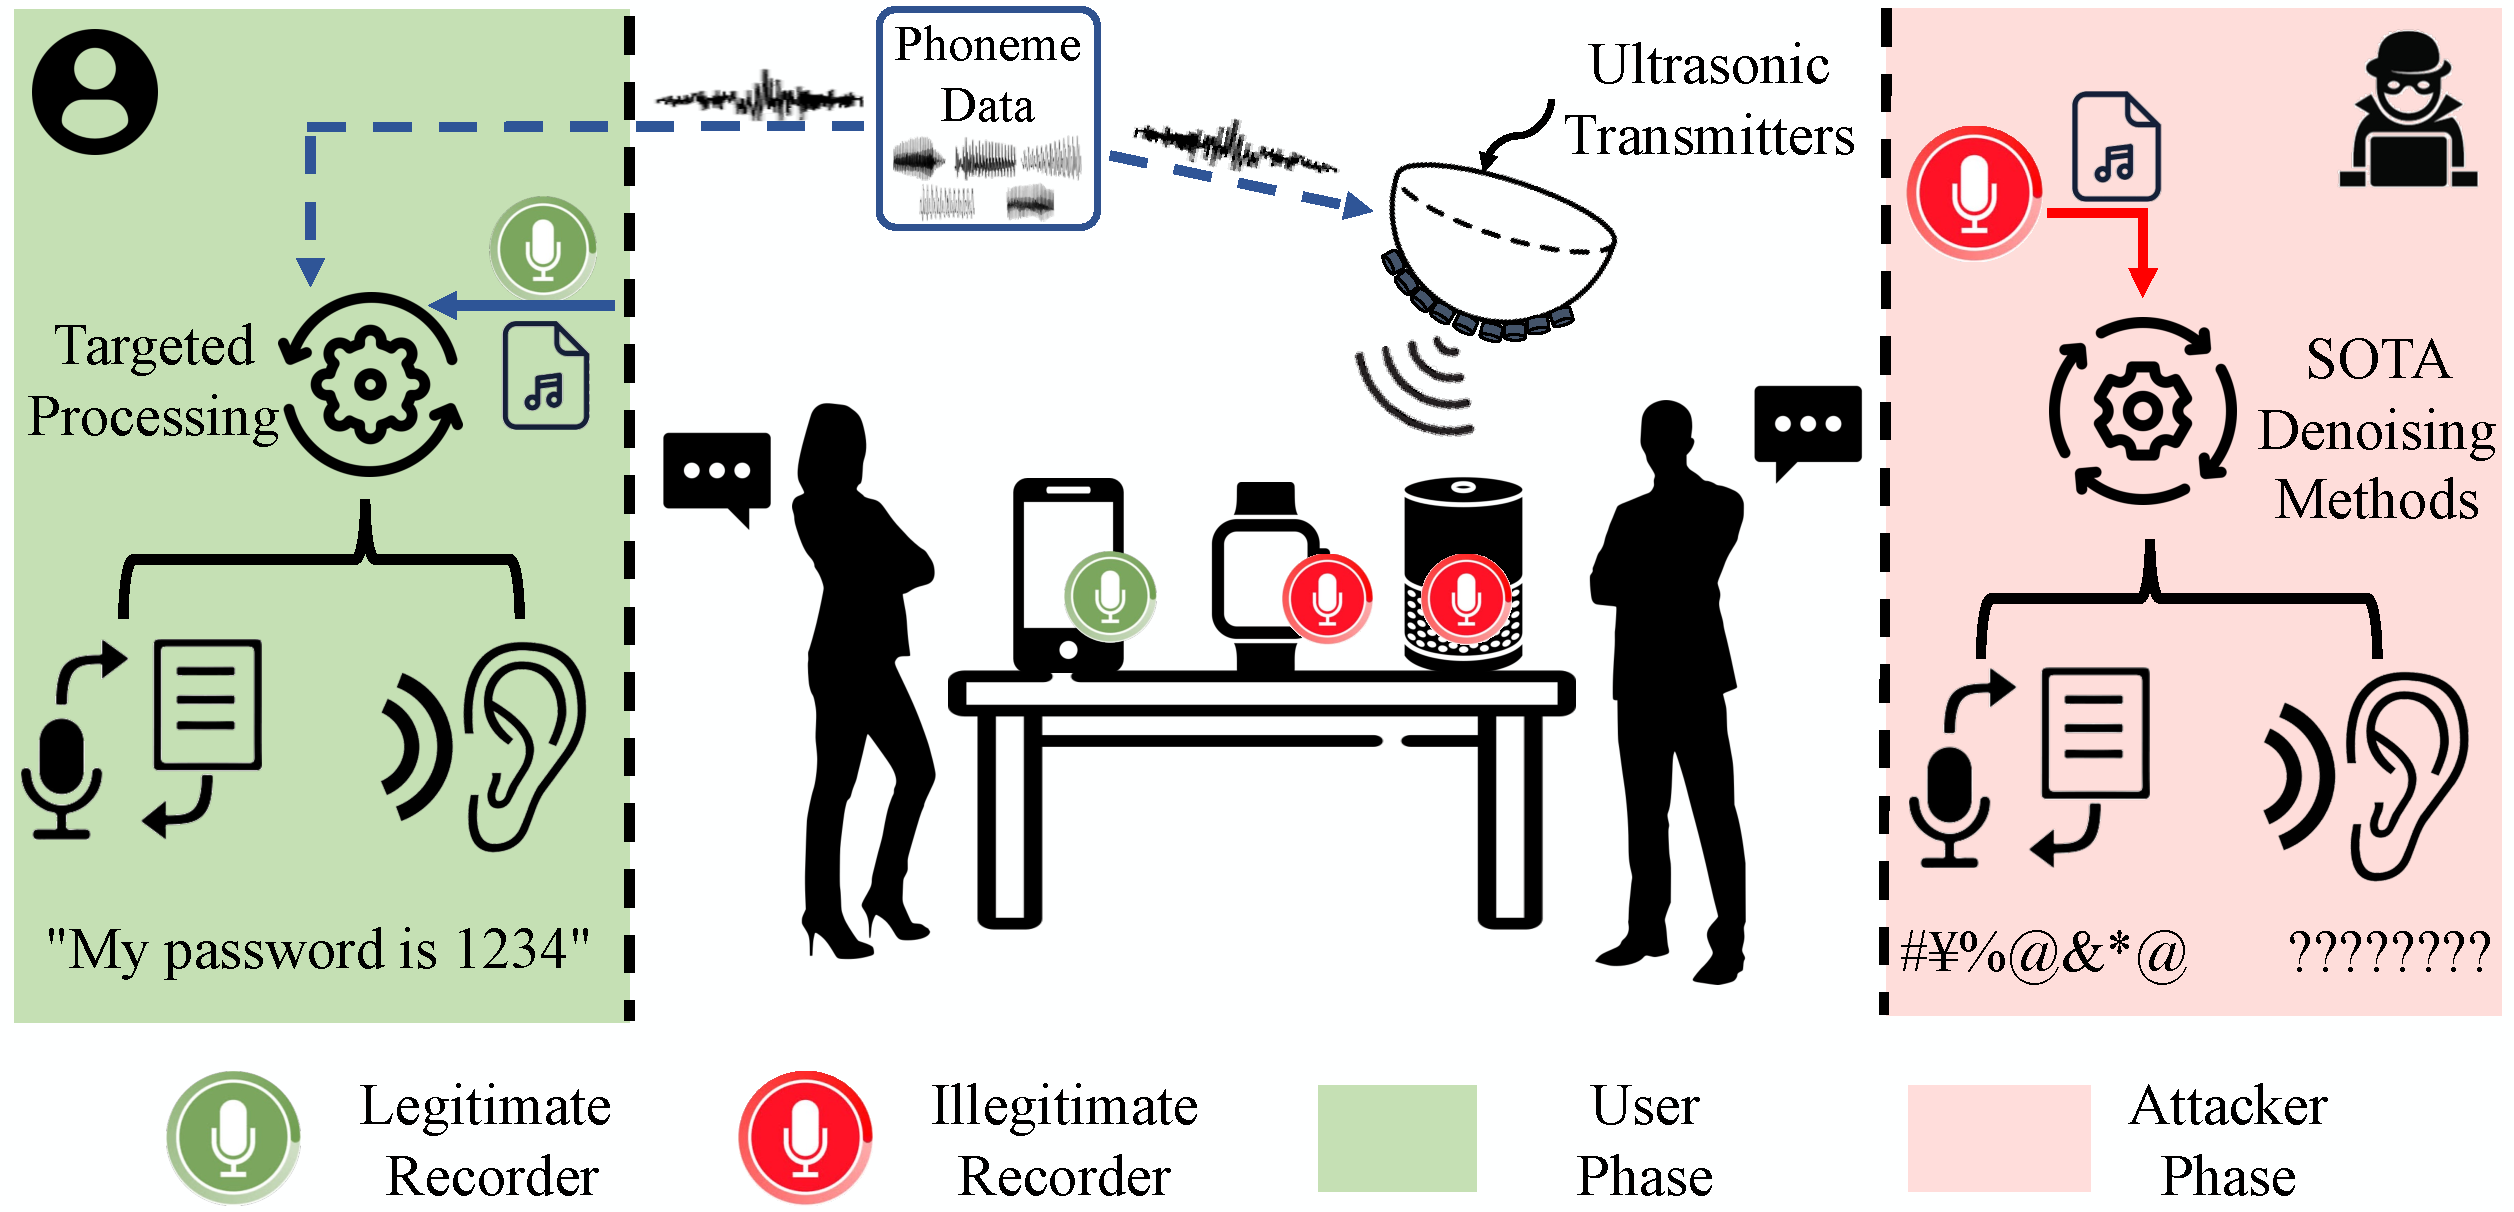
\includegraphics[width=\linewidth]{images/introduction_system.pdf}
    \caption{Anti-Eavesdropping with user-controlled recording.}
    \label{fig:introduction_system}
    \vspace{-7mm}
\end{figure}

The critical condition of voice privacy shows the necessity of anti-eavesdropping techniques. However, existing solutions fall far short of needs.
For example, Project Alias~\cite{alias} and Paranoid Home Wave~\cite{Paranoid} inject white/chatter noise into microphones to prevent potential sound monitoring. 
Nevertheless, to reduce the disturbance caused by the audible noise, users have to attach the noise transmitter to the microphone to lower the noise energy, which is not applicable in some scenarios.
GhostTalk~\cite{GhostTalk} applies electromagnetic interference (EMI) to induce noises to internal circuits of microphones, but the EMI could affect nearby devices like cardiac pacemakers, which could lead to unexpected results.

To overcome these difficulties, researchers attempt to jam recorders in other ways. 
In 2017, Roy and Zhang et al. reveal a new side channel in microphones that can inject audible signals into microphones with inaudible ultrasound~\cite{10.1145/3133956.3134052,backdoor}. The key point is to modulate the target audible signal on an ultrasonic carrier before sending it to the microphone. Once being received, the modulated signal will be demodulated automatically because of the non-linearity, as shown in Figure~\ref{fig:nonlinearity_in_microphone}. Its acceptable transmission distance ($>$2m) and neglectable influence on nearby users and devices make this method a promising solution for jamming voice recorders.

Based on this, Chen~et al. implement a bracelet-like wearable to emit ultrasound noises, achieving good jamming coverage by utilizing users' irregular arm movements~\cite{CHI}. Li~et al. propose Patronus~\cite{patronus} that can disturb recorders with carefully designed noises and adopts an iron reflection layer to extend coverage. Gao~et al. design MicFrozen~\cite{gao_cancelling_2023}, which reduces signal-to-noise ratio (SNR) of recordings by cancelling voice signals and adding coherent noises. Sun~et al. design MicShield~\cite{sun_alexa_2020} which provides selective jamming for smart speakers based on wake word detection.

We systematically analyze existing studies and reveal their limitations, as shown in Table~\ref{tab:overview}. First, most of them adopt simple-form noises such as White Gaussian Noise (WGN) and random frequency noise, which achieve audio jamming solely based on high power. On the one hand, the high power ultrasound could harm the human ear~\cite{human_ultrasound_tolerance}. On the other hand, the non-linearity also exists in transmitters~\cite{211283}, so the energy of the transmitted noise should be controlled within a certain range to avoid emitting audible noises. These two issues create a central dilemma between jamming coverage and usability. Besides, these simple-form noises can be easily removed by noise reduction techniques, thus cannot prevent the leakage of privacy thoroughly~\cite{Walker2021Evaluating}. For the works utilizing speech-based noise~\cite{gao_cancelling_2023}, they employ continuous speech signals, which gives a chance to remove them from recordings with speech separation techniques. This fact is devastating for an anti-eavesdropping application as an adversary is very likely to apply state-of-the-art (SOTA) denoising techniques or even targeted noise removal methods before privacy extraction. In addition, most of existing works do not support authorized recording, which limits the usage scenario.

\begin{table}[]
    \caption{An Overview of Anti-Eavesdropping Systems}
    \resizebox{\columnwidth}{!}{
        \begin{threeparttable}
        \begin{tabular}{cccccc}
            \toprule
            System     & Noise Form    &\begin{tabular}[c]{@{}c@{}}Commercial\\ ASRs~$\dagger$\end{tabular}  & \begin{tabular}[c]{@{}c@{}}SOTA \\ Enh.$~\dagger$\end{tabular}& \begin{tabular}[c]{@{}c@{}}Specialized\\ Enh.$~\dagger$\end{tabular} & \begin{tabular}[c]{@{}c@{}}Recording\\Support\end{tabular}\\ \midrule

            MicFrozen~\cite{gao_cancelling_2023}   & Speech~*  & \ding{51}             & \ding{51}       & \ding{55} & \ding{55}               \\
            MicShield~\cite{sun_alexa_2020}     & WGN           & \ding{51}             & \ding{55}         &      \ding{55}& \ding{55}        \\
            Roy et al.~\cite{backdoor} & WGN~*     & \ding{55}              & \ding{55}         & \ding{55}    &  \ding{55}   \\
            Patronus~\cite{patronus}   & Random Freq.~*  & \ding{51}             & \ding{55}         & \ding{51}    & \ding{51}          \\
            Chen et al.~\cite{CHI}      & WGN           & \ding{51}             & \ding{51}       & \ding{55}         &  \ding{55}    \\
            This work     & Phoneme~* & \ding{51}             & \ding{51}       & \ding{51}     & \ding{51}         \\ \bottomrule
        
        \end{tabular}

        \begin{tablenotes}
            \small 
            \item \textit{Note: * in Noise Form means generated based-on, not exactly the same. \ding{55} in $\dagger$ columns means that the authors have not conducted relevant experiments.}
            
        \end{tablenotes}
    \end{threeparttable}
    }
    \label{tab:overview}
    \vspace{-6mm}

\end{table}

In this paper, we propose an anti-eavesdropping system that achieves effective and reliable jamming with support for authorized recording in real-world privacy-preserving scenarios. Instead of solely relying on high power, we explore the idea of informational masking, which achieves jamming by disturbing the signal structure in recordings. Specifically, we design a new type of jamming noise that contains multiple phoneme sequences. When jammed by our noise, the phoneme structure of the speech signal would be greatly obscured. Since phonemes are the basic units of sound for distinguishing words, the chaotic phoneme pattern makes the speech signals hard to understand. Moreover, our noise shows inherent robustness against both existing SOTA and targeted-trained denoising methods. The discrete phonemes in our noise make denoising methods fail to disentangle the genuine speech elements from distracting ones due to their high similarity. We encourage readers to listen to audio examples at the demo website~\footnote{\url{https://github.com/desperado1999/InfoMasker}. Relevant codes will also be released here.}. The utilization of information masking also relaxed the requirement on high energy, and we further address the challenge on increasing the jamming range without losing inaudibility. At last, we propose a transformer-based content recovery method to provide support for authorized recordings.

In general, we summarize our contributions as follows:
\begin{itemize}
    \item We propose a new type of jamming noise, named Phoneme-Based Audio Jamming Noise, based on the idea of informational masking.
    \item We design and implement a system based on our noise, which can prevent eavesdropping while preserving recording permission for authorized users.
    % \item We optimize several aspects of the ultrasound-based noise transmission method to make it suitable for our noise and practical in real-world scenarios
    \item We conduct comprehensive experiments to evaluate our system from different aspects. The results prove the high effectiveness and robustness of our system and show its usability in real-world scenarios.
\end{itemize}